% \chapter{Relativistic Heavy Ion Collisions}
% \section{RHIC and LHC}
% \section{Collision Energy and Geometry}
% \section{Kinematic Variables}
% \section{QGP Evolution}
% \section{Detection of Collision Products}
% \section{Detection of QGP Signatures}
% \subsection{Dilepton Production}
% \subsection{Bjorken Energy Density}
% \subsection{Collective Flow}
% \subsection{Strangeness Enhancement}
% \subsection{Jet Quenching}
% \subsection{Photon Production}
% \section{Transverse Energy}
% \section{RHIC Beam Energy Scan Program}

\chapter{Relativistic Heavy Ion Collisions}\label{ch:RHI-collisions}
%%%%%%%%%%%%%%%%%%%%%%%%%%%%%%%%%%%%%%%%%%%%%%%%%%%%%%%%%%%%%%%%%%%%%%%%%%%%%%%%%%%%%%%%%%%%%%
The experimental evidence for the QGP comes from the collisions of heavy nuclei. Some of its signatures are described in section \ref{section:signatures}. Physicists proposed the existence of such matter since as far back as 1984, when nuclei were accelerated and collided with stationary targets \cite{Gyulassy:2004vg}. They were able to agree on a conclusive discovery of this matter during the 2000s, after colliding accelerated nuclei with other such nuclei or smaller species (protons, deuterons) at unprecedented energies and with improved detection schemes \cite{Ritter:2004xj}. With further increases in collision energies and enhancements in detector technology, modern accelerator facilities provided additional evidence and estimates of some of the properties as well as the dynamics of the evolution of the QGP. The following sections describe two such facilities, the physics of the collisions, and what happens after the collisions.

\section{RHIC and LHC}
The Relativistic Heavy Ion Collider (RHIC) is located in Upton, New York in the premises of the Brookhaven National Laboratory (BNL). Its construction started in 1991 and was completed in 1999. Figure \ref{fig:RHIC_layout} shows the layout, at the time of construction, of the collider along with the Alternating Gradient Synchrotron (AGS) complex and the locations of the original four detectors: Solenoidal Tracker At RHIC (STAR), Pioneering High Energy Nuclear Interaction eXperiment (PHENIX), Phobos, and BRAHMS (Broad RAnge Hadron Magnetic Spectrometers). Phobos, BRAHMS, and PHENIX were decommissioned after the completion of their science objectives, but STAR is still operational. The AGS was part of BNL before the construction of the RHIC, and its capabilities were augmented with the construction of the AGS Booster in 1991.
\begin{figure}[h]
  \centering
  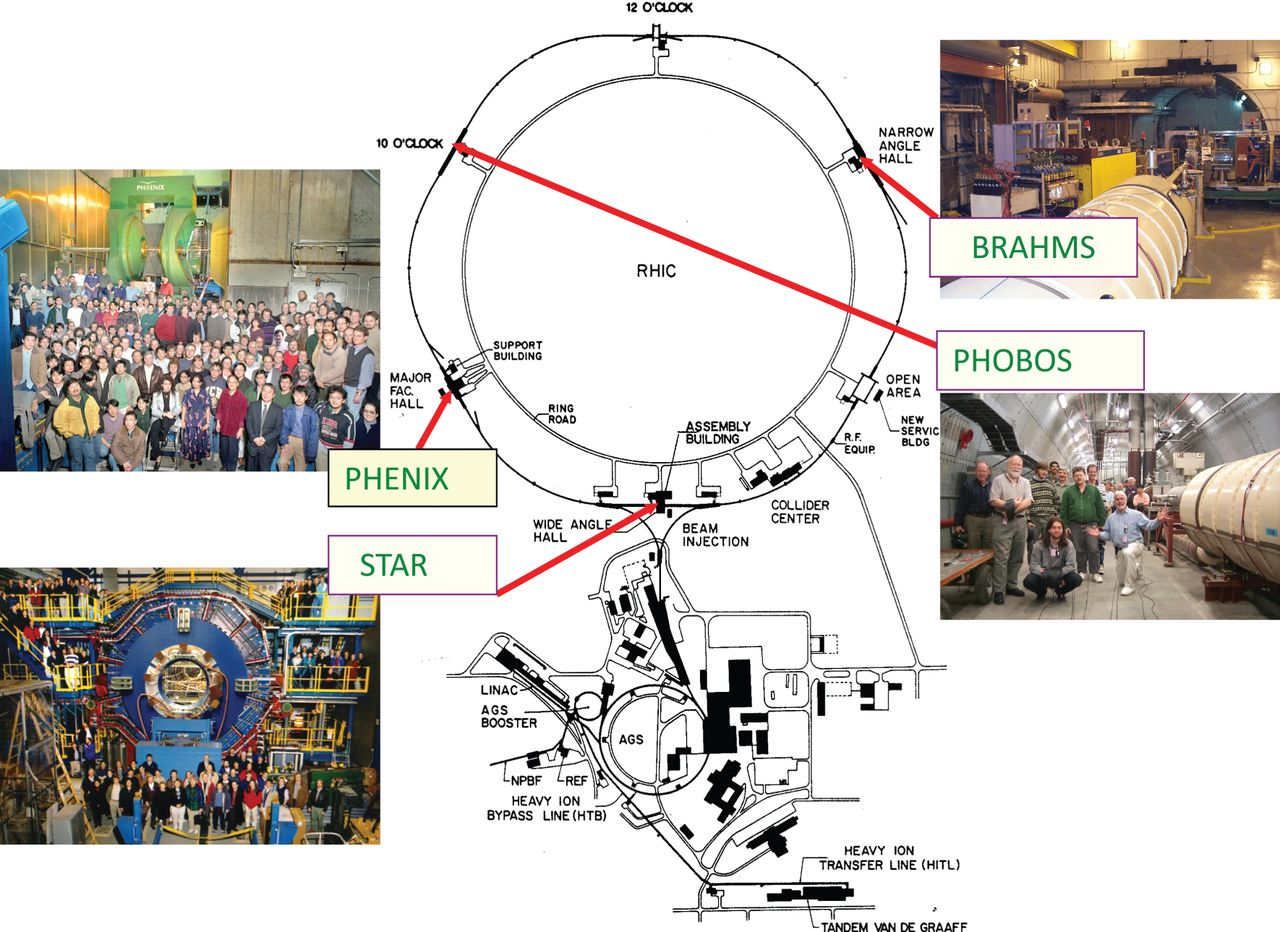
\includegraphics[width=6.5in]{figures/RHIC_Layout.jpeg}
  \caption{Initial layout of the RHIC \cite{doi:10.1093/ptep/ptu093}.}\label{fig:RHIC_layout}
\end{figure}

Heavy ion beams in RHIC are created in a series of steps before collision. In case of gold ions, a pulsed sputter source produces negatively charged ions, which are stripped of some of their electrons with a foil on the positive end of the high-voltage Tandem Van de Graff. The ions are now positively charged and are accelerated to 1MeV/u toward the negative terminal of the Tandem. Upon exiting it, some more stripping takes place. The bending magnets then selectively deliver +32 charge states of the ions to the Booster Synchrotron, which accelerates them to 95MeV/u and strips them to a +77 charge state before injecting them to the AGS. The AGS accelerates them to 10.8 GeV/u and strips them of the remaining two electrons at the exit. The gold ions are then injected through the AGS-to-RHIC Beam Transfer Line to the two RHIC rings. These rings carry beams moving in opposite directions and intersect at six symmetric locations in the 3.8 km circumference. The original four detectors are located in four of these six locations where the beams undergo head-on collisions.

The Large Hadron Collider (LHC) is located underground (between 45m and 170m) beneath the France-Switzerland border near the city of  Geneva. The two rings of the collider were constructed between 1998 and 2008 by the European Organization for Nuclear Research (CERN) in the 26.7 km circular tunnel originally housing CERN's Large Electron-Positron collider. Analogous to the RHIC, the LHC gets its beams prepared by a series of machines in the CERN accelerator complex. The collisions occur at the locations of the four big LHC experiments: Compact Muon Solenoid (CMS), A Toroidal LHC ApparatuS (ATLAS), Large Hadron Collider beauty (LHCb) experiment, and A Large Ion Collider Experiment (ALICE). ALICE is dedicated to the study of heavy-ion collisions \cite{1748-0221-3-08-S08001}.
%%%%%%%%%%%%%%%%%%%%%%%%%%%%%%%%%%%%%%%%%%%%%%%%%%%%%%%%%%%%%%%%%%%%%%%%%%%%%%%%%%%%%%%%%%%%%%%%

\section{Collision Energy and Geometry}\label{geometry}
What happens in the aftermath of a collision depends on how much energy is available at the time of the collision as well as the geometry of the collision. The collision energy is determined by the collider configuration. The geometry of the collision is deduced as the collision $centrality$, as described later in this section, through the estimation of the charged particle multiplicities ($N_{ch}$) resulting from the collisions.  

In collision experiments, it is convenient to use a reference frame in which the net momentum of the pair of colliding species is zero. This frame is called the center-of-mass frame. In this frame, the total energy of the species in the two beams is a function of the number of nucleons and the center-of-mass energy per nucleon. The collision energy is reported as the center-of-mass energy per nucleon pair, $\sqrt{s_{NN}}$. %The magnitude of this quantity constrains the species that can be produced from any collision.

%!!!!!!!!!!!!!!! Details in:
%1. https://arxiv.org/pdf/1604.02651.pdf
%2. http://www.phys.hawaii.edu/~teb/phys481l/relkin.pdf
%3. http://edu.itp.phys.ethz.ch/hs10/ppp1/PPP1_4.pdf

RHIC has the unique capability of colliding species at a range of energies spanning almost two orders of magnitude. Table \ref{table:RHIC_specs} lists the collision energies produced so far at RHIC for various collision systems. The LHC boasts the highest amount of collision energy for any collider on earth. It collided species (p+p, p+A, Pb+Pb) at a center of mass energy up to 2.76 TeV per nucleon pair at the end of 2010. At the end of 2015, 5.02 TeV Pb+Pb and 13 TeV p+p collisions were successfully completed \cite{FOKA2016154}.

\begin{table}[h!]
\centering
\begin{tabular}{||c c||}
%\tabletypesize{\scriptsize}
%\rotate
\hline
Collision system & $\sqrt{s_{NN}}(GeV)$ \\ [0.5ex]
\hline
\hline
p+p & 200, 510 \\
d+Au & 19.6, 39, 62.4, 200 \\
Cu+Cu & 62.4 \\
Cu+Au &  200 \\
p+Au & 200 \\
$^3$He+Au & 200 \\
Au+Au & 7, 7.7, 9, 20, 62, 130, 200 \\ [1ex]
\hline
\end{tabular}
\caption{Colliding species and associated collision energies at RHIC \cite{McGlincheyPrivateCommunication}.}
\label{table:RHIC_specs}
\end{table}


In general, any collision between two nuclei is not perfectly head-on. Some collisions are close to being head-on and are called central collisions. Some are glancing and are called peripheral collisions. %The amount by which a collision is central is quantitatively represented by a variable called centrality. 
By convention, 0\% is the centrality of a perfectly head-on collision and 100\% is that of the least head-on, i.e., the most peripheral collision. More central collisions generally produce more particles \cite{Connors:2017ptx}.

The centrality is estimated through a model-based correlation between $N_{ch}$ and the impact parameter, defined as the distance between the centers of the two nuclei at the time of their maximum overlap. The Monte Carlo based model, for instance, assumes that all nucleons travel in straight lines along the beam direction \cite{Loizides:2014vua} and that they collide if they overlap \cite{Miller:2007ri}. $N_{ch}$ is assumed to scale with the number of participants and the number of binary collisions. The distribution of this quantity is then fit to the data and the fraction of the overlap is estimated from the observed $N_{ch}$ value. 5\% of all collisions with the highest $N_{ch}$ values, for example, are then referred to as being 0-5\% central \cite{Connors:2017ptx}.
% In practice, each collision event is deducted to belong to a specific centrality bin. For instance, 0-5\% would be the centrality for an identified $N_{ch}$ value which would be the minimum charged particle multiplicity produced by at most 5\% of the total number of collisions. This identification of the $N_{ch}$ value is often acheived by using the a Glauber model \cite{Connors:2017ptx,Miller:2007ri}.

Figure \ref{fig:mid-central_collision} illustrates the aftermath of a mid-central collision, i.e, a collision in which about half of the volume of each of the nuclei intersects the other.%............. add brief discussion of Glauber model and STAR centrality determination.............
	\begin{figure}[h]
	  \centering
	  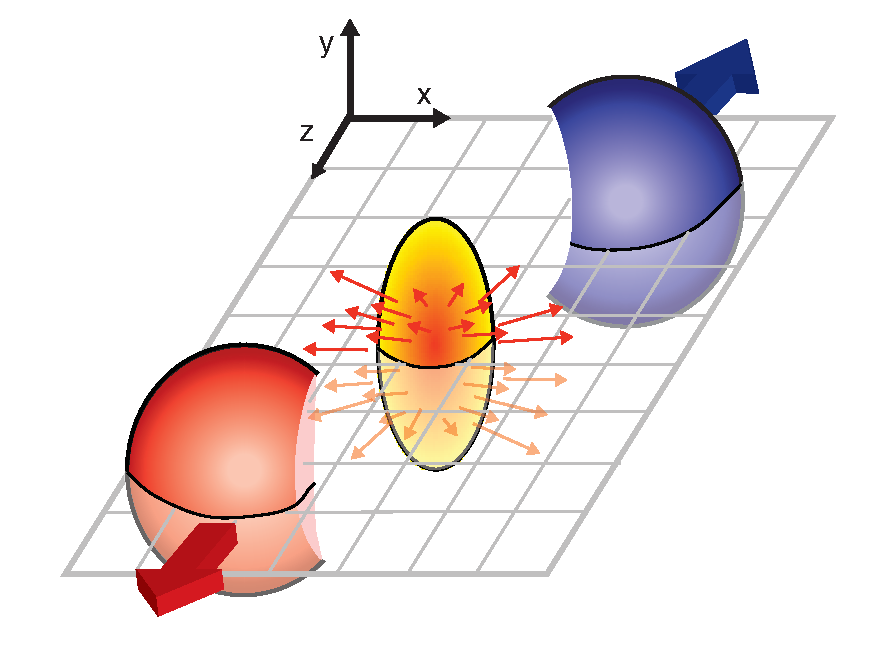
\includegraphics[width=4.5in]{figures/flow_elliptic_init_v4.pdf}
	  \caption{An illustration of a mid-central collision of two nuclei traveling in the z direction. The X-axis is parallel to the line joining the centers of the two nuclei at the time of collision \cite{Connors:2017ptx}.}\label{fig:mid-central_collision}
	\end{figure}

The collision of two nuclei can be modeled as collisions of the constituents that make up the nuclei. The nucleons that take part in the collisions and are called participants. The rest of the nucleons are known as spectators. Figure \ref{fig:part_spec} illustrates the distribution of participants and spectators in two colliding nuclei.% Expectedly, the number of participants is more in more central collisions.
\begin{figure}[h]
  \centering
  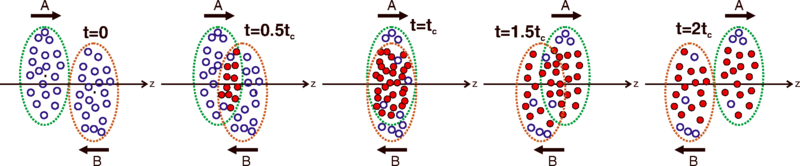
\includegraphics[width=6.5in]{figures/part_spec_Vovchenko.png}
  \caption{An illustration of a collision consisting of participants (solid red) and spectators (open blue) within the colliding nuclei labeled A and B. $t_{c}$ denotes the time of maximum overlap of the two nuclei. The apparent narrowing of the volumes of the nuclei in the z-direction is due to Lorentz contraction \cite{PhysRevC.90.044907}.}\label{fig:part_spec}
\end{figure}
%%%%%%%%%%%%%%%%%%%%%%%%%%%%%%%%%%%%%%%%%%%%%%%%%%%%%%%%%%%%%%%%%%%%%%%%%%%%%%%%%%%%%%%%%%%%%%%%

\section{QGP Evolution}
\begin{figure}[h]
  \centering
  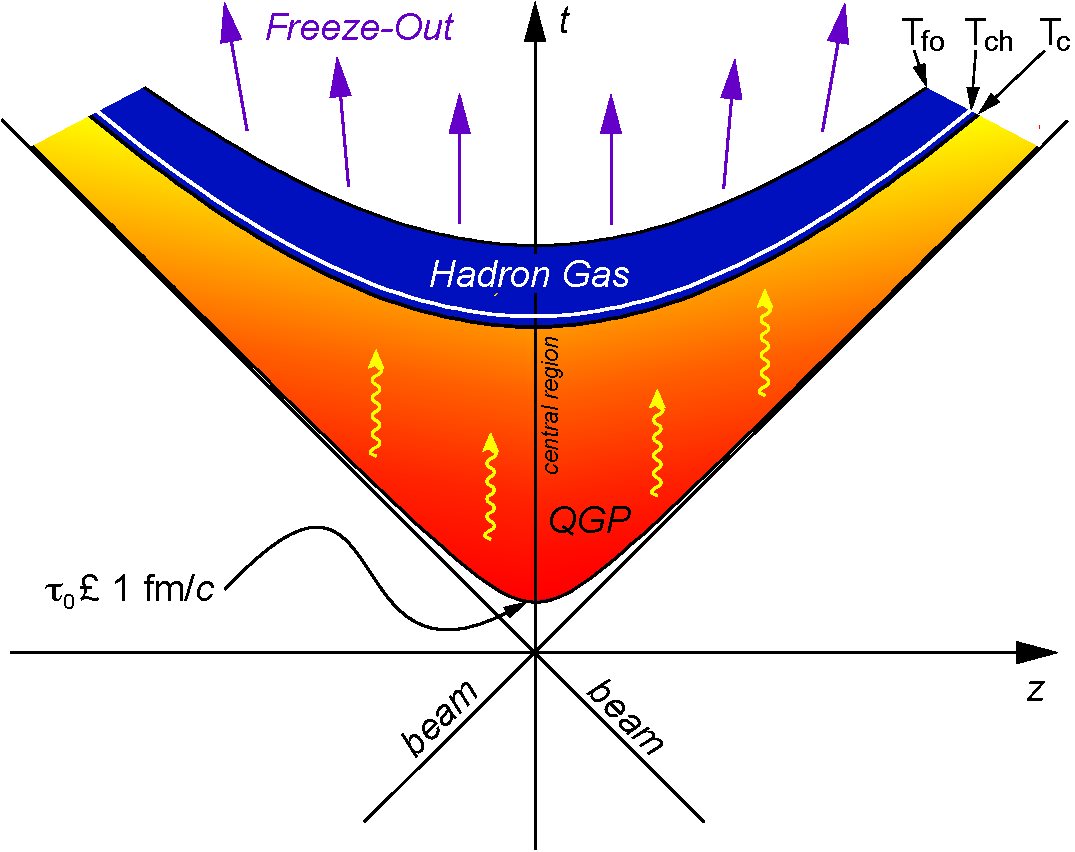
\includegraphics[width=5.5in]{figures/LightCone1_color-crop_NThesis.pdf}
  \caption{Evolution of the QGP represented in a lightcone diagram. $\tau_{0}$ denotes the formation time of the QGP. $T_{c}$ is the critical temperature of the transition from the QGP to the hadron gas phase. $T_{ch}$ and $T_{fo}$ stand for the temperatures at, respectively, chemical freeze-out and thermal freeze-out \cite{Connors:2017ptx}.}\label{fig:lightcone}
\end{figure}
The evolution of the QGP is shown in a lightcone diagram in figure \ref{fig:lightcone} \cite{Connors:2017ptx}. The initial state of the colliding nuclei is not precisely known and is the topic of research for upcoming experiments. During the collision, the participants scatter off of each other while the spectators keep traveling almost unperturbed in their original direction. The immediate aftermath of a central collision of heavy ions at RHIC and LHC energies is the formation of a hot fireball. This fireball evolves in time to form a liquid-like medium of quarks and gluons. This medium attains a local equilibrium and remains in such a state, depending on the collision energy, for about 1-10 fm/c. This equilibrium is broken as the liquid QGP evolves by expanding and cooling to attain a density and temperature at which the medium undergos hadronization followed by a chemical freeze-out to form a hadron gas. The particle ratios are fixed after the chemical freeze-out. Collisions between the constituents of this gas become scant as it evolves with further expansion and cooling, and the hadrons undergo a thermal freeze-out to attain their final energies and momenta \cite{Connors:2017ptx}.

\section{Detection of Collision Products}\label{subsection:detection}
%%%The final state particles emit in all directions around the collision site. The symbol $\theta$ is used to denote the polar angle of the direction, i.e., the angle with respect to the beam axis, of a particle. However, it is more convenient to use a different quantity, called the rapidity, to describe the particle's direction.
Detectors are placed around the collision site to perform measurements on the final state particles emitting from the thermal freeze-out of the medium. These measurements typically include the reconstruction of the particle tracks, estimation of the the types of particles, and the momenta and energies they carry.

Generally, a tracking detector surrounds the collision site, and there are particle identifiers followed by calorimeters around it. A magnetic field is applied parallel to the beam direction around the collision site. Due to this orientation of the magnetic field, the spectators traveling parallel to it move roughly undeflected and the final state charged particles with components of velocity transverse to the beam axis get deflected around the beam axis with radius given by
\begin{equation}\label{eqn:larmor}
r = \frac{p_{T}}{qB},
\end{equation}
where $p_{T}$ is the transverse momentum of the particle, $q$ is its electric charge, and $B$ is the applied magnetic field.
Two kinds of detectors most relevant to this thesis, tracking detectors and calorimeters, are described in chapter \ref{ch:measurement}.

\section{Detection of QGP Signatures}\label{section:signatures}
%http://iopscience.iop.org/article/10.1088/0954-3899/25/3/013/meta, and: 

The existence and properties of the QGP in the aftermath of high-energy heavy-ion collisions can be probed using different techniques relevant to several theoretical characteristics of the medium. No signature can alone be used to claim the production of the QGP, and some of the probes, which should be interpreted together, are described below.


%Analyses of experimental results have thus far provided signatures of the formation of matter with partonic degrees of freedom at the early stages of the collisions. Such signatures include suppression of high monentum hadrons, known as jet quenching, because the QGP is nearly opaque to colored probes, and large azimuthal anisotropies, indicating that the medium is a liquid of quarks and gluons \cite{PhysRevC.96.044904}?????. %Experiments also reveal the initial energy density of this matter to be about two orders of magnitude larger than that of low energy nuclear matter -- comfortably more than the deconfinement phase transition critical density predicted by lattice QCD \cite{2005PrPNP..54..443J}.

%The state of the colliding nuclei before the collision at LHC and top RHIC energies has indications of being a Color Glass Condensate -- strongly interacting, weakly coupled highly coherent gluonic matter \cite{1742-6596-458-1-012024}. The characteristics of the initial states of these nuclei affect the partonic distributions within the nuclei and ultimately the products of the collision. The collision products are also affected by variables such as the initial energy and entropy densities of the partonic matter \cite{2005PrPNP..54..443J}.

%Different observables can be used to study different aspects of heavy ion collisions. The charged particle multiplicity, $\langle N_{ch} \rangle$, is a global variable that relates to the entropy production during the collision (analysis note). The transverse energy, $E_{T}$, a global variable related to $\langle N_{ch} \rangle$, provides information about the conversion of the initial beam-direction kinetic energy into energy flowing in the transverse direction after the collision. Together, the studies of the fluctuation of the $\langle N_{ch} \rangle$ and the $E_{T}$ pseudorapidity [footnote] density with respect to the beam energy and the collision centrality [footnote] help probe the characteristics of the initial conditions at the time of the collision. One can study, for instance, the distinctions between models based on quark participants against those based on nucleon participants [analysis note]. These quantities can also lead to the rough estimate of the initial energy density through the use of the Bjorken formula \cite{2012ARNPS..62..361M}:
%\ref{eqn:Bjorken}
%\begin{equation}\label{eqn:Bjorken}
%\epsilon \geq \frac{\frac{dE_{T}}{d\eta}}{\tau_{0}\pi R^{2}} = \frac{3}{2}\langle \frac{E_{T}}{N} \rangle \frac{\frac{dN_{ch}}{d\eta}}{\tau_{0}\pi R^{2}}
%\end{equation}
%The transverse energy and the charged particle pseudorapidity densities have conventionally been calculated by using the transverse energy measurements obtained from calorimeters. This thesis details the use of particle spectra, reported as $\frac{d^{2}N}{dydp_{T}}$, from Au+Au collisions at RHIC to calculate the same global variables and serve as a method to cross check the ones involving calorimeters.
\subsection{Bjorken Energy Density}
%mostly pg 271 to 275 in \cite{Wilde:2012wc}
In 1983, J.D. Bjorken\cite{PhysRevD.27.140} prescribed a formula to use the final state particles to estimate the initial energy density, $\epsilon_{0}$, in a nucleus-nucleus collision. With slight changes in the original formula, the energy density is estimated by:
	\begin{equation}\label{eqn:bjorken}
	\epsilon_{0} = \frac{1}{\tau_{0}A_{T}}\langle\frac{dE_{T}}{dy}\rangle,
	\end{equation}
where $\tau_{0}$ is the formation time of the QGP, $A_{T}$ is the transverse area of the intersection of the two nuclei, and $\langle\frac{dE_{T}}{dy}\rangle$ is the mean transverse energy per unit rapidity. $\tau_{0}$ is model-dependent and is normally estimated to be $~1 fm/c$. $A_{T}$ depends on the centrality of the collision and can be estimated using the Glauber model discussed earlier. $\langle\frac{dE_{T}}{dy}\rangle$ is found from the measurement of the transverse energy carried by the final state particles from the collision and is the central theme of this thesis. Details about it are in the following chapters.
The estimate of the initial energy density from the Bjorken formula is an underestimate of the maximum energy density because the measured $dE_{T}/dy$ is an average over the system as it undergoes expansion and cooling. It can be compared with the QCD prediction of the critical energy density \cite{Adam:2139456} to check if the results from a collision imply the achievement of the critical physical condition required for the phase transition \cite{2005PrPNP..54..443J}. Experiments show that ultra-relativistic heavy ion collisions are capable of producing energy densities comfortably higher than those predicted by QCD \cite{Adam:2139456}.
%Experiments reveal it to be about two orders of magnitude larger than that of low energy nuclear matter -- comfortably more than the deconfinement phase transition critical density predicted by lattice QCD \cite{2005PrPNP..54..443J}.

\subsection{Elliptic Flow}
The evolution of the medium produced in relativistic heavy ion collisions can be well described under the framework of relativistic hydrodynamics \cite{SCHENKE2017105,2014NuPhA.926...92S}. This description indicates the presence of a collective flow of a locally thermalized liquid. The angular distribution of the momenta of the final state particles emitted out of the collectively flowing system can be decomposed into a Fourier expansion in its azimuthal components. The second harmonic coefficient, $\nu_{2}(y,p_{T})$, of this decomposition characterizes what is known as the elliptic flow \cite{2001PhLB..503...58H}. The magnitude of the elliptic flow from a non-central collision represents the anisotropy in azimuthal momentum space of the thermalized post-collision system \cite{2011NJPh...13e5008S}.
%In normal matter, the speed of sound is generally more in solid than in liquid and more in liquid than in gas. This is because it its proportional to the ......
The elliptic flow of the medium, as a function of the momentum or the kinetic energy in the transverse direction, points towards quarks, rather than hadrons, being the relevant degrees of freedom in the QGP. Figure \ref{fig:v2Scaling1} shows $v_{2}$ as a function of the transverse momentum and the transverse kinetic energy for identified particles. The spectra scale consistently at lower values of both $p_{T}$ and $KE_{T}$. However, they branch out as mesons and baryons at higher values: $p_{T} \gtrsim 2 GeV/c and KE_{T} \gtrsim 1 GeV$. Figure \ref{fig:v2Scaling2}, on the other hand, is similar to figure \ref{fig:v2Scaling1}, with the exception that both the axes have quantities that are normalized by the number of quarks, $n_{q}$. In this case, the $KE_{T}$ spectra strongly exhibits a scaling which is more comprehensively consistent with the number of quarks than in case of figure \ref{fig:v2Scaling1}. This universal quark-number scaling can be interpreted as the degrees of freedom of the system being quark-like \cite{2007PhRvL..98p2301A}.
	\begin{figure}[h]
	  \centering
	  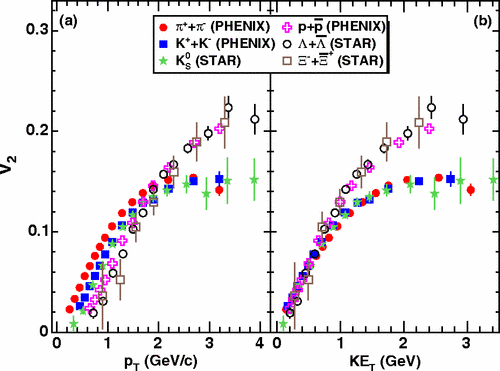
\includegraphics[width=4.5in]{figures/v2Scaling1.png}
	  \caption{Minimum-bias Au+Au ($\sqrt{s_{NN}} = 200 GeV$) elliptic flow spectra for identified particles: (a) $v_{2}$ vs $p_{T}$ and (b) $v_{2}$ vs $KE_{T}$ \cite{2007PhRvL..98p2301A}.}\label{fig:v2Scaling1}
	\end{figure}
	
	\begin{figure}[h]
	  \centering
	  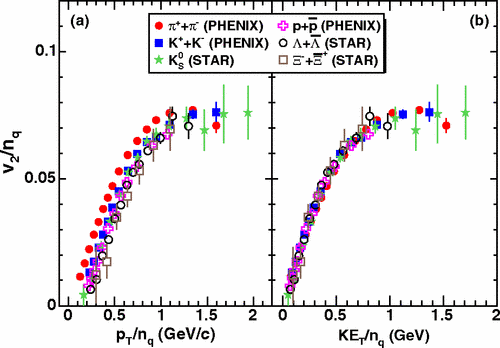
\includegraphics[width=4.5in]{figures/v2Scaling2.png}
	  \caption{Minimum-bias Au+Au ($\sqrt{s_{NN}} = 200 GeV$) elliptic flow spectra for identified particles: (a) $\frac{v_{2}}{n_{q}}$ vs $\frac{p_{T}}{n_{q}}$ and (b) $\frac{v_{2}}{n_{q}}$ vs $\frac{KE_{T}}{n_{q}}$ \cite{2007PhRvL..98p2301A}.}\label{fig:v2Scaling2}
	\end{figure}

\subsection{Prompt and Thermal Photons}
Most of the photons observed after relativistic heavy ion collisions are the results of the decay of the neutral pion into two gammas. %The remaining photons can be divided into direct photons from hard scatterings, which can be calculated in perturbative QCD, and thermal photons.
When these photons are subtracted from the observations, the remaining photons are called direct photons \cite{PAQUET2016409}. These direct photons are produced within the fireball via different mechanisms as discussed below.
\begin{figure}[h]
  \centering
  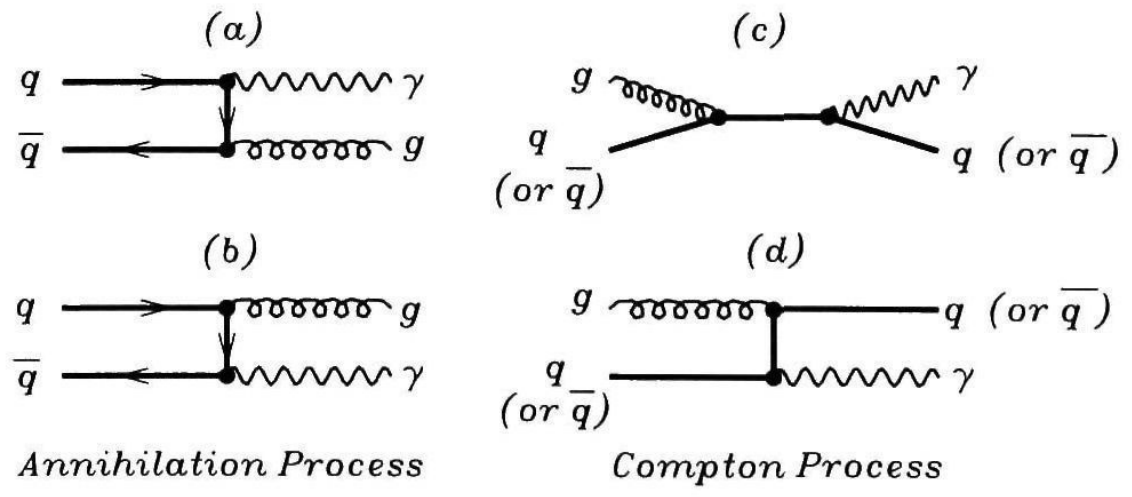
\includegraphics[width=6.5in]{figures/directPhotons.PNG}
  \caption{Feynman diagram representing the production of photons from quarks and gluons. $(a)$ and $(b)$ represent annihilation processes, whereas $(c)$ and $(d)$ represent Compton processes \cite{wong1994introduction}.}\label{fig:directPhotons}
\end{figure}

In the QGP, a quark and an antiquark can annihilate to produce a photon and a gluon. It is also possible for the pair to annihilate and produce two photons, but the probability of this process is smaller than the former by about two orders of magnitude. Furthermore, a quark (or an antiquark) can interact with a gluon to produce an antiquark (or a quark) and a photon, a process analogous to Compton scattering in QED. The photons produced from the hard scattering processes between the partons are called prompt photons, and their multiplicity scales with the number of binary collisions. Photons can also be produced due to scatterings of partons within the thermalized medium, and these photons are called thermal photons. The nature of the $p_{T}$ distribution is different in this case as the emission process mimics blackbody radiation. This difference helps distinguish these photons from the direct photons produced by partonic interactions. Just like the leptons described in the previous section, the photons produced in the QGP can only interact with the medium electromagnetically. Therefore, they undergo minimal scattering before being detected, and hence can be used to probe the thermodynamical state of the medium at the time of their creation \cite{wong1994introduction,PAQUET2016409,Wilde:2012wc}.

\subsection{Strangeness Enhancement}
% http://shodhganga.inflibnet.ac.in/bitstream/10603/37674/11/11_chapter%202.pdf
The interacting nuclei carry no net strangeness before colliding, and so an observation of strange and multi-strange particles after the collision can be used to probe the properties of the post-collision medium \cite{1742-6596-455-1-012005}. Strangeness can also be produced in hadron-hadron collisions. However, it is enhanced in nucleus-nucleus collisions \cite{Behera:2012eq}. This is interesting because it possibly indicates a restoration of chiral symmetry, which is a topic of ongoing research: in the zero baryon chemical potential limit, lattice QCD calculations reveal a transition of QCD matter between a phase with broken and one with restored chiral symmetry \cite{ refId0}. Chiral symmetry restoration has the implication of all the flavors of quarks losing their masses \cite{Sazdjian:2016hrz}. Hence, when chiral symmetry is restored, it is more feasible to produce strange quarks, for instance, which have higher masses than the light quarks, up and down, in a state of broken chiral symmetry. Chiral symmetry restoration is not the only possible reason for the production of many strange quarks. It is also feasible to produce strange quarks as long as the temperature of the system is above the strange flavor mass scale, and so it carries effects of the system temperature. This is exemplified by the ratio of the production of the strange kaons to that of the non-strange pions, which are the most abundant hadrons produced from nucleus-nucleus collisions: kaon yield increases more rapidly than pion yield does as the temperature increases \cite{wong1994introduction}.% This can be shown mathematically by treating the system as a hadron gas in thermal and chemical equilibrium that follows the Bose-Einstein distribution, but it is beyond the scope of this thesis

% https://arxiv.org/pdf/1612.04078.pdf
% more: https://indico.cern.ch/event/555216/contributions/2414536/attachments/1394348/2125058/Bratkovskaya_WWND-2017.pdf

\subsection{Jet Quenching}
A scattering event in which the participants transfer a large amount of their original momenta is called hard scattering. The products of the scatterings are called jets. %Ultimately, jets are what are recognized by a jet finder algorithm as jets. 
In heavy-ion collisions, most hard scatterings are the results of two partons from the opposite nuclei scattering off each other. These partons can lose their momenta by strongly interacting with the enhanced gluon fields in a QGP medium. Therefore, the properties of the jets, as carried by the final state hadrons, should be different for collisions that produce the QGP as compared to those that do not, and hence they can be used as signatures and probes of QGP. Figure \ref{fig:jets} illustrates the quenching of jets that have to travel long distances in the medium. %Details about the forms of interaction of the hard partons with the QGP is beyond the scope of this thesis. 
%%Formalisms developed to study jet quenching due to radiative and collisional energy losses are detailed in \cite{2015IJMPE..2430014Q}. 
	\begin{figure}[h]
	  \centering
	  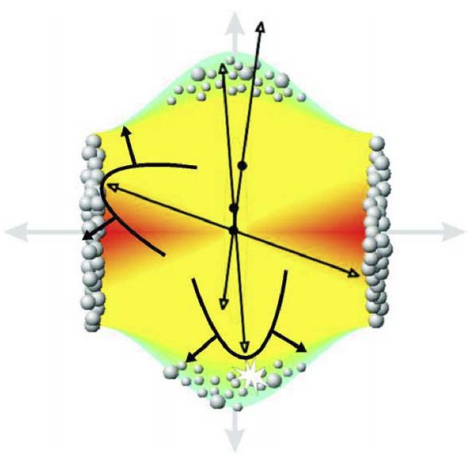
\includegraphics[width=4.5in]{figures/jets.PNG}
	  \caption{Illustration of jet quenching. Two jets are produced from each of the hard scatterings occuring at the locations of the solid dots. Jets originating closer to the initial surface are more probable to propagate outside the medium, as shown. Jets opposite to them interact with the medium, losing their energy and resulting in bow front shock waves \cite{STOCKER2005121}.}\label{fig:jets}
	\end{figure}
	
The nuclear modification factor, $R_{AA}$, is the ratio of the cross section for particle production in nucleus-nucleus collisions scaled by the number of binary nucleon-nucleon collisions divided by the cross section in proton-proton collisions.  It is shown in Fig. \ref{fig:Raa} for several different particle species, demonstrating substantial suppression of high momentum particles. This shows that the medium is nearly opaque to colored probes.
	\begin{figure}[h]
	  \centering
	  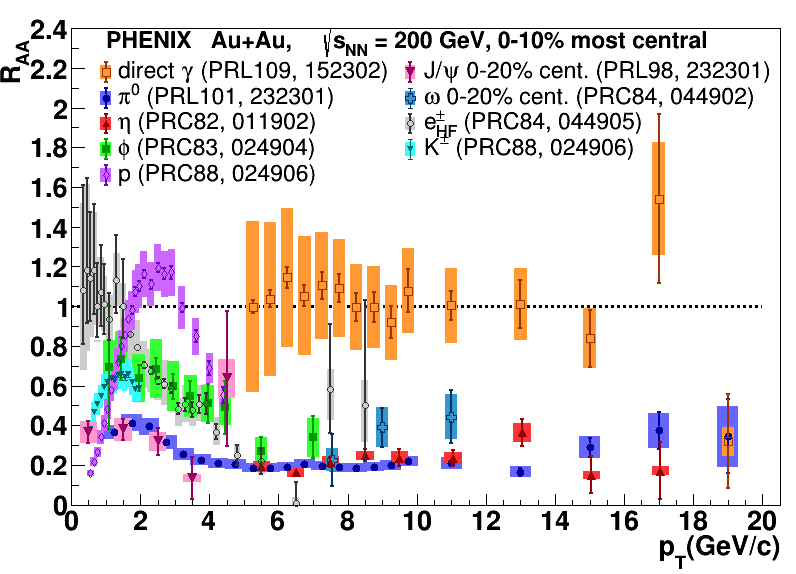
\includegraphics[width=6.5in]{figures/Raa.PNG}
	  \caption{$R_{AA}$ from PHENIX for direct photons \cite{Afanasiev:2012dg}, $\pi^0$ \cite{Adare:2008qa}, $\eta$ \cite{Adare:2010dc}, $\phi$ \cite{Adare:2015ema}, $p$ \cite{Adare:2013esx}, J/$\psi$ \cite{Adare:2006ns}, $\omega$ \cite{Adare:2011ht}, $e^{\pm}$ from heavy flavor decays \cite{Adare:2010de}, and $K^{\pm}$ \cite{Adare:2013esx}.  This demonstrates that colored probes (high-$p_{T}$ final state hadrons) are suppressed while electroweak probes (direct photons) are not at RHIC.}\label{fig:Raa}
	\end{figure}
	
%The interaction of the jets in the QGP medium can be in the form of gluon bremsstrahlung or parton collision.

\section{The Beam Energy Scan Program}
The RHIC, in 2010, started a multi-phase Beam Energy Scan (BES) program to study the QCD phase diagram. Between 2010 and 2011, during the exploratory phase I of the BES program, the collider provided Au+Au collisions at 7.7, 11.5 (not completed in PHENIX), 19.6, 27, and 39 GeV. Together with the data formerly collected by the RHIC at higher collision energies, BES phase I data can scan the interval from 450 MeV to 20 MeV in $\mu_{B}$ space \cite{1742-6596-455-1-012037, LUO201675}. One of the things that can be studied with the data associated with this region of the phase space is the possibility of a ``turn-off of new phenomena already established at higher RHIC energies"\cite{1742-6596-455-1-012037}. Results corresponding to the high-$\mu_{B}$ region might provide evidence of a first order phase transition, and possibly the critical point \cite{LUO201675}.
% (https://drupal.star.bnl.gov/STAR/starnotes/public/sn0493)

The manifestation of such phenomena might be in terms of the fluctuations or other properties of the post-collision system. One can, for instance, study the scaling of the energy density after the collision with the longidutional energy at the time of the collision, $\sqrt{s_{NN}}$, for which one needs to measure the transverse energy. This can be done in multiple ways using a detector like STAR or PHENIX that is made up of sub-systems such as the Time Of Flight (TOF) detectors, Time Projection Chambers (TPCs)/Time Expansion Chambers, and calorimeters. The next chapter describes the measurement of transverse energy using BES data from PHENIX calorimeters. Also, the next chapter and the ones after it contain the procedures and the results of the analysis of the BES data from STAR using the identified particle spectra.

%\section{Transverse Energy}
%\section{RHIC Beam Energy Scan Program}
